\begin{figure}[tp!]
	\centering
	\begin{subfigure}[t]{\linewidth}
	\begin{subfigure}[t]{0.33\linewidth}
		\centering
		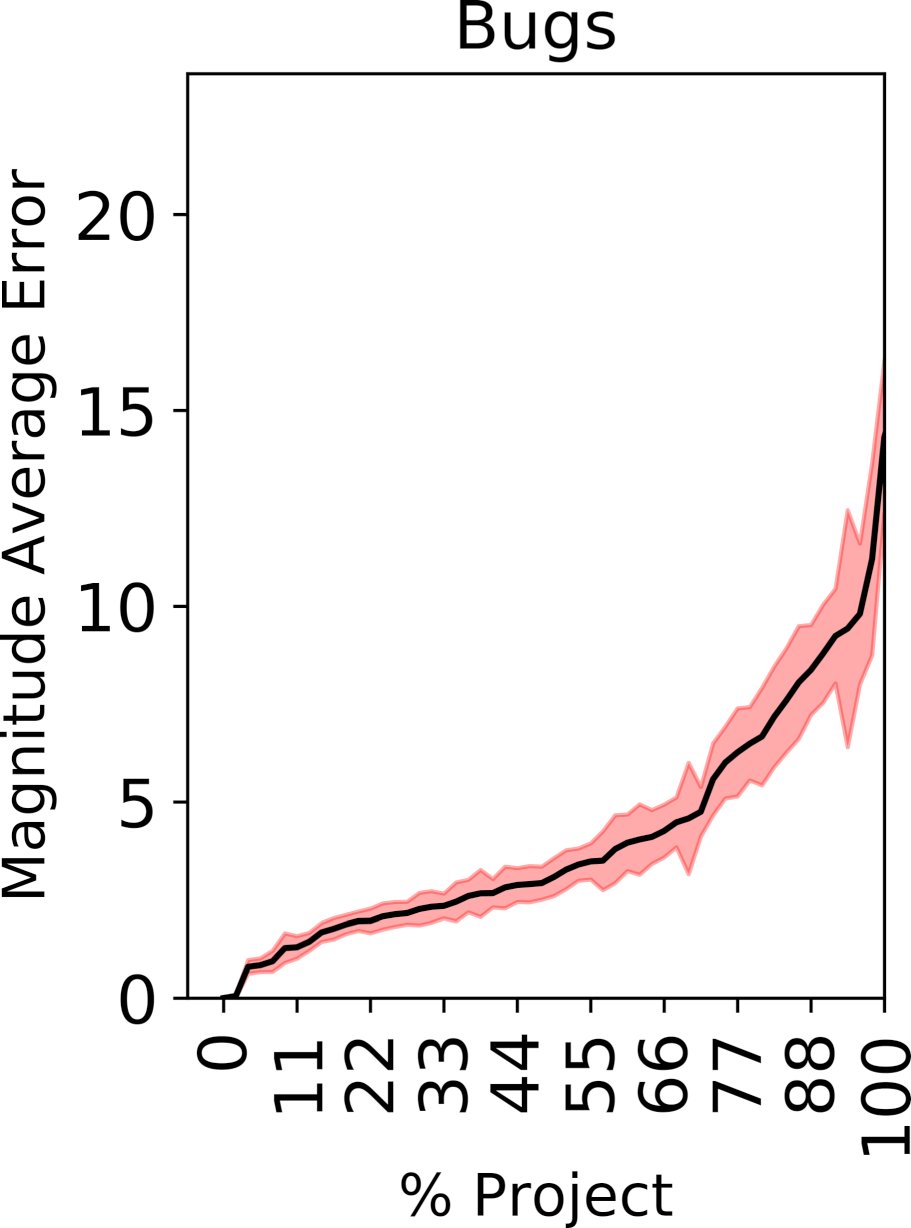
\includegraphics[width=\linewidth]{images/RQ1/inhouse/Bugs.png}
	\end{subfigure}%
	~
	\centering
		\begin{subfigure}[t]{0.33\linewidth}
		\centering
		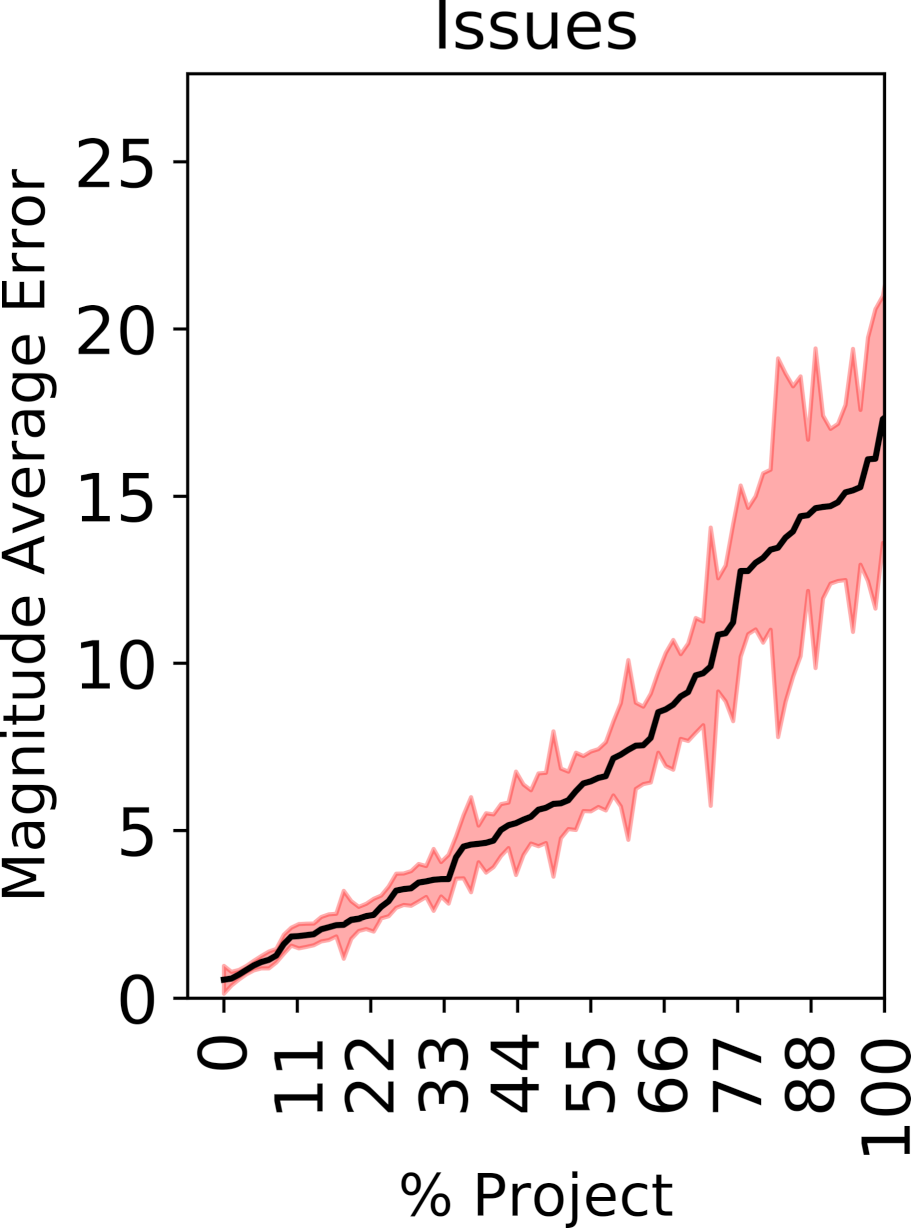
\includegraphics[width=\linewidth]{images/RQ1/inhouse/Issues.png}
	\end{subfigure}%
	~
	\centering
		\begin{subfigure}[t]{0.33\linewidth}
		\centering
		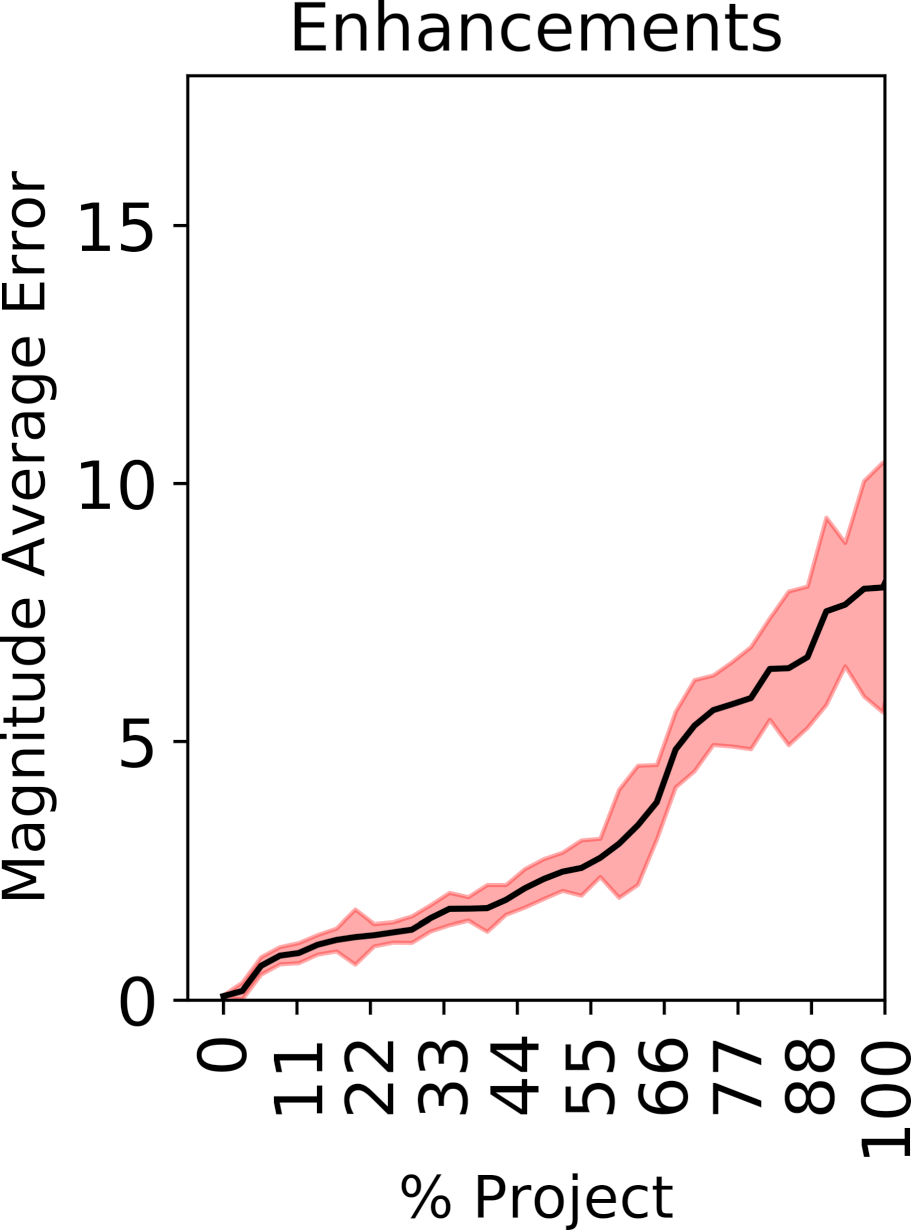
\includegraphics[width=\linewidth]{images/RQ1/inhouse/Enhancements.png}
	\end{subfigure}%
	\caption{171 Proprietary Datasets}
	\end{subfigure}
	\\
	\begin{subfigure}[t]{\linewidth}
	\begin{subfigure}[t]{0.33\linewidth}
	\centering
	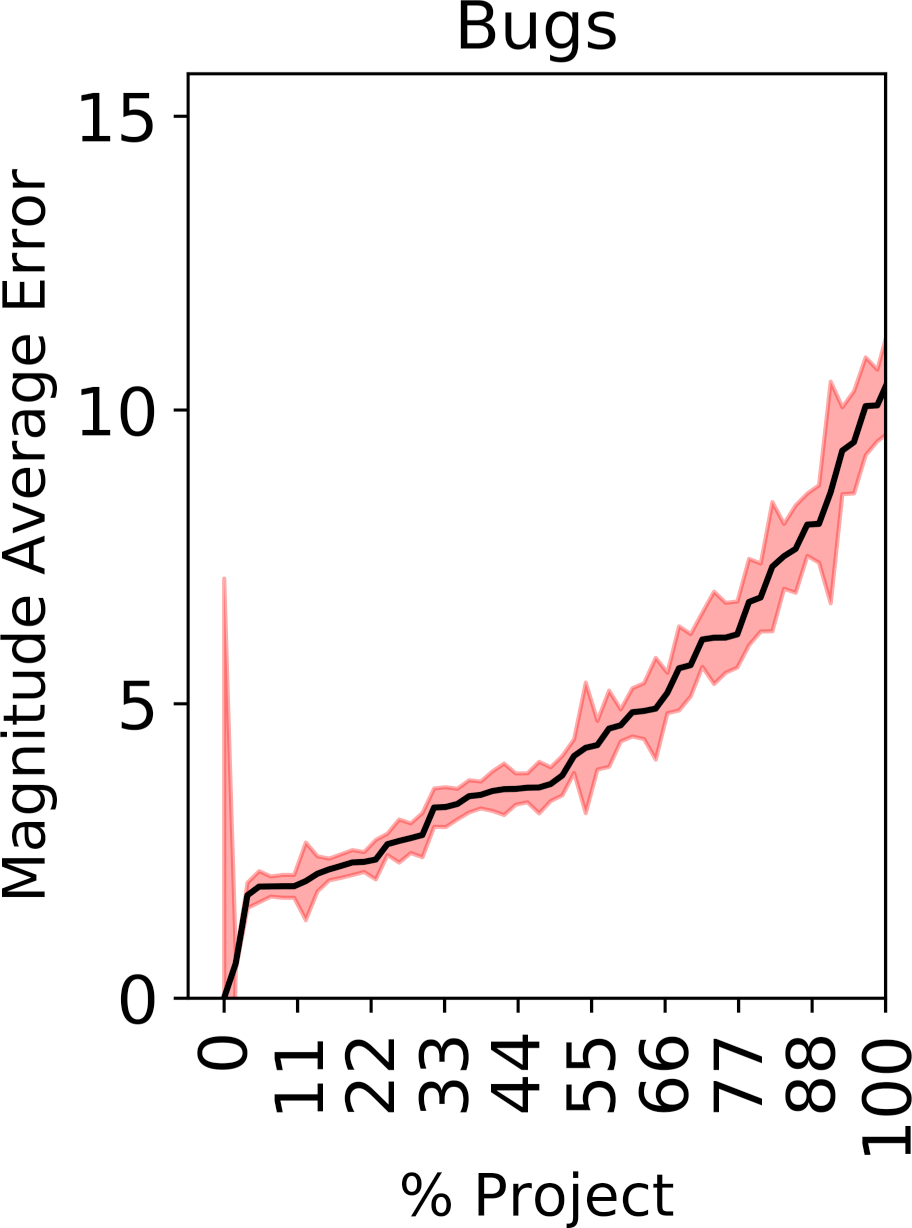
\includegraphics[width=\linewidth]{images/RQ1/opensrc/Bugs.png}
	\end{subfigure}%
	~
	\centering
	\begin{subfigure}[t]{0.33\linewidth}
		\centering
		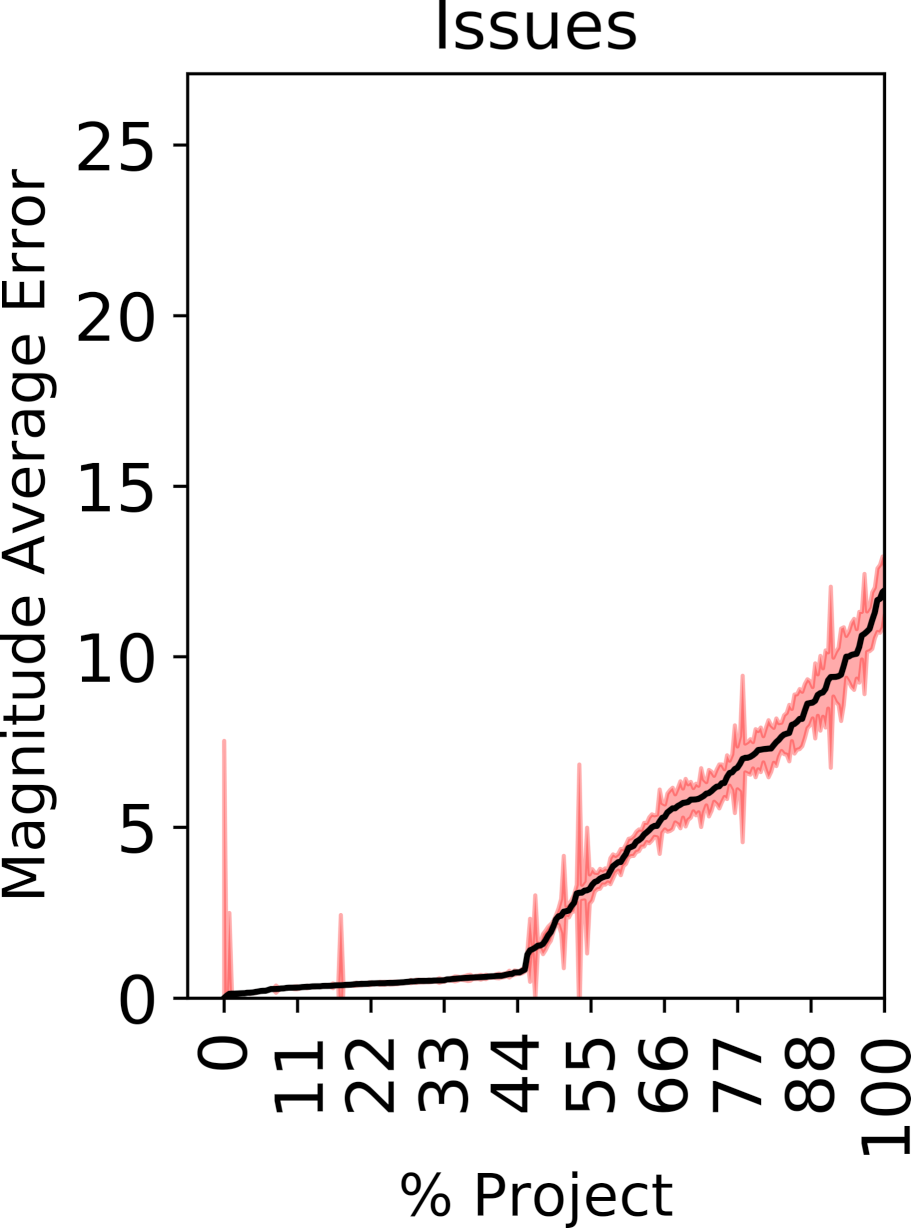
\includegraphics[width=\linewidth]{images/RQ1/opensrc/Issues.png}
	\end{subfigure}%
	~
	\centering
	\begin{subfigure}[t]{0.33\linewidth}
		\centering
		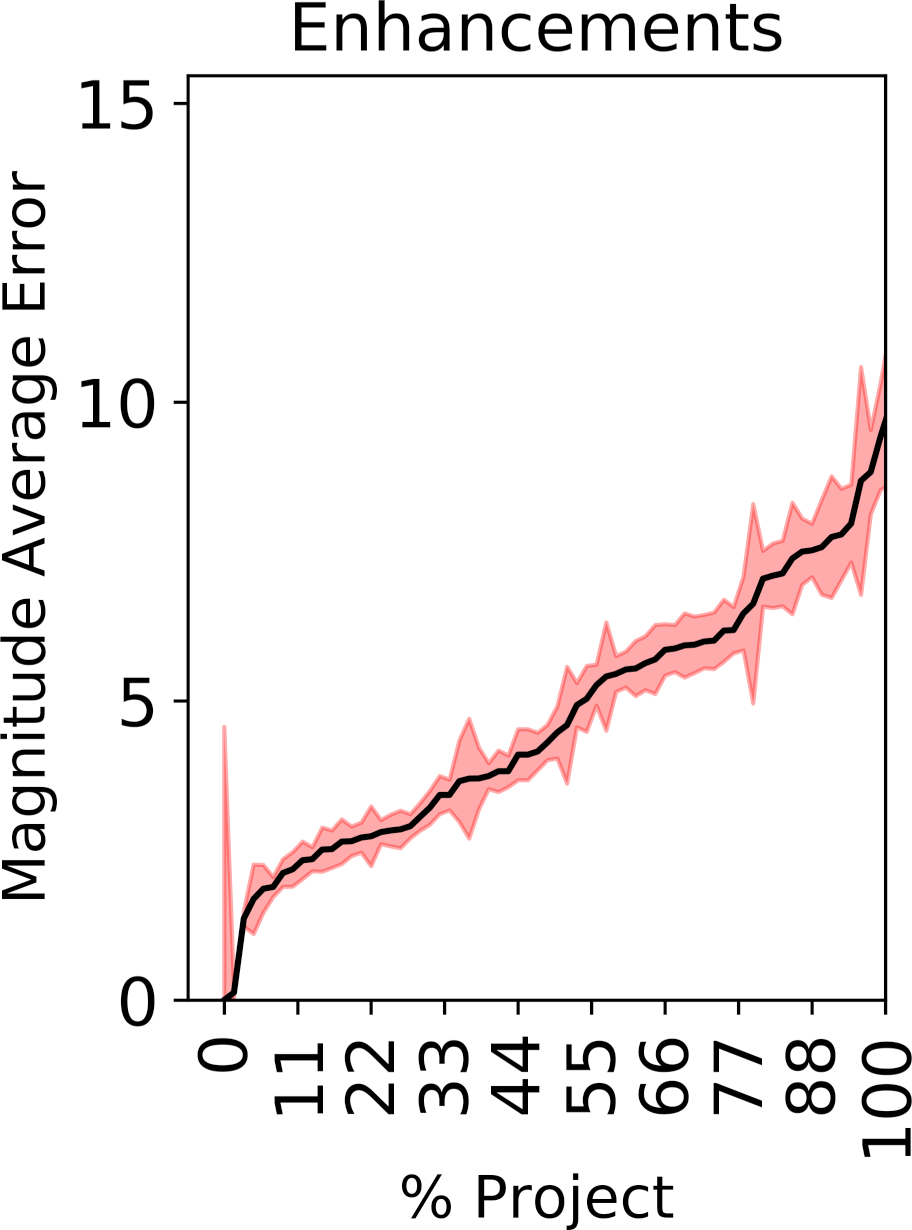
\includegraphics[width=\linewidth]{images/RQ1/opensrc/Enhancements.png}
	\end{subfigure}%
	\caption{671 Opensource datasets}
	\end{subfigure}
	\caption{This figure verifies the existence of temporal trends in issues, bugs, and enhancements. The low magnitude of average error (MAE) values show that time series forecasting with ARIMA can be performed on these attributes.}
	\label{fig:rq1}
\end{figure}
